In the following, SLIM is used in various configurations as a surrogate for modelling the present values of benefits of two fictitious insurance tariffs from the TRAIL.X (TRustworthy Artificial Intelligence in Life Insurance) research project \citep{msginsurit.16.03.2023}. The results are interpreted and the fidelity is compared with the MBT algorithms GUIDE, MOB and CTree.

\subsection{Data set K2204}
The data set K2204 contains data for a (fictitious) endowment insurance tariff. With this tariff, a single benefit is paid both in the event of survival and death of the policyholder. The data set includes the features sex (1 = male, 0 = female), age and duration and the two targets benefit present value (BPV) and premium present value (PPV). The targets were modelled using two different black box models.  
In the following, only the BPV is considered. The results for the PBV are very similar (interpreted the other way round) and can be found in the appendix.
Since the data set with 5994 observations is rather small, all observations were used for training. For this data set, we therefore only consider the training performance in the surrogate models.
A special characteristic of K2204 is a correlation between the features Age and Duration, as can be seen in Figure \ref{fig:ins_corr_age_duration}. When interpreting a MBT for this data set, it must therefore be taken into account that a split with regard to one of the features always has an influence on the value range of the other feature.

\begin{figure}[!htb]
    \centering    
    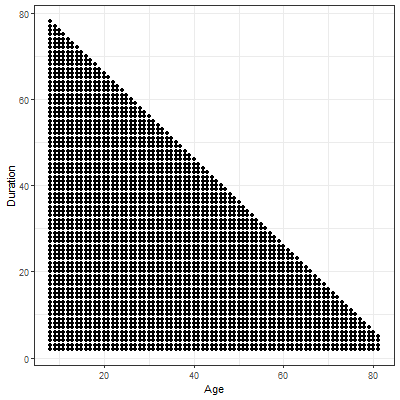
\includegraphics[width=5cm]{Figures/insurance_use_case/k2204_BPV/corr_age_duration.png}
    \caption{Features Age and Duration in the K2204 data set}
    \label{fig:ins_corr_age_duration}
\end{figure}


\subsubsection{Shallow MBTs with linear models}
In a first step, SLIM was fitted as surrogate to the black box predictions of BPV (BPV\_pred) with linear regression models in the nodes. The maximum depth was set to 3 and an improvement in the objective of at least 0.1 of the previous improvement was set as prepruning parameter.
 The resulting tree is shown in Figure \ref{fig:ins_slim_lm_tree}.

 \begin{figure}[!htb]
     \centering     
     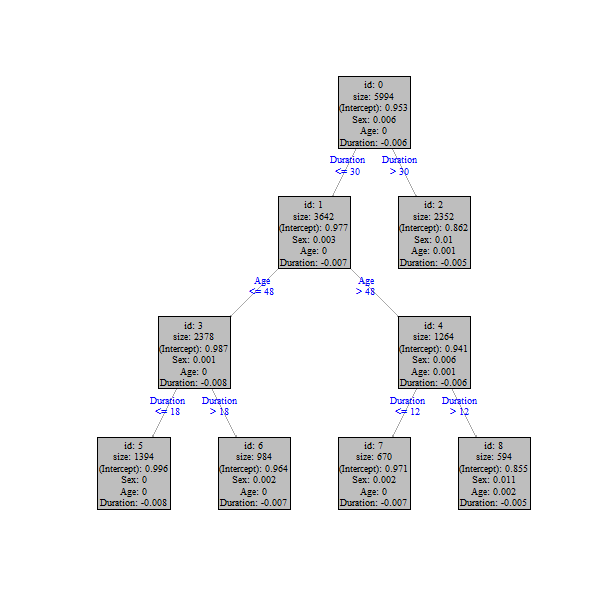
\includegraphics[width = 14cm]{Figures/insurance_use_case/k2204_BPV/slim_lm_tree.png}
     \caption{SLIM tree for K2204 with linear models}
     \label{fig:ins_slim_lm_tree}
 \end{figure}

Basic observations across all subregions are:
\begin{itemize}
    \item Gender male has a positive effect on BPV\_pred
    \item Age has a positive effect on BPV\_pred
    \item Duration has a negative effect on BPV\_pred
\end{itemize}

The strength of the effects, however, differs in the different subregions found by SLIM.
The five leafnodes can be roughly divided into two regions with similar effects:
\begin{itemize}
    \item Region 1 (Nodes 2,8): High Duration ($30$) or high Age ($>48$) and medium Duration (between $13$ and $30$)
    \item Region 2 (Nodes 5,6,7): Low - medium Duration with low Age or high Age with low Duration ($\leq 12$)
\end{itemize}

In Region 1 Sex male and Age have a higher positive effect on  BPV\_pred than in region 2. The negative effect of duration, on the other hand, is smaller in region 1. This indicates a non-linearity of duration.

If SLIM is fitted as a standalone model instead of a surrogate model in the same configuration, the differences in the split points are very small. This indicates that the black box model captures the underlying relationships very well. The corresponding tree is shown in the appendix in Figure \ref{fig:app_ins_slim_lm_standalone_tree}.

In the following, the fidelity of the different MBT with algorithms with linear models is compared. For this purpose, all four algorithms were fitted with a maximum depth of 3. For SLIM and GUIDE, $impr$ is set to $0.05$ and for MOB and CTree $alpha$ is set to $0.05$. Furthermore, a minimum nodesize of 200 observations is required.
The MBTs are compared with a baseline model, which is a linear regression model on the entire feature space. In addition to the $R^2$ and the MSE, the mean absolute error (MAE) and the maximum absolute error (max AE) were included as measures of fidelity. The max AE is particularly important here, as it is strictly regulated in order not to discriminate against any individual. 
The results are listed in table \ref{tab:ins_k2204_lm_surrogates_perf}. It shows that all MBTs achieve considerable improvement over the baseline model.

\begin{table}[!htb]

\caption{Fidelity of K2204 linear baseline model and linear MBTs}
\centering
\begin{tabular}[t]{l|r|r|r|r|r}
\hline
  & r2 & MSE & MAE & max AE & n leaves\\
\hline
linear baseline model & 0.985101 & 0.000201 & 0.011393 & 0.064709 & 1\\
\hline
SLIM & 0.999233 & 0.000010 & 0.002272 & 0.020526 & 8\\
GUIDE & 0.999276 & 0.000010 & 0.002142 & 0.020526 & 8\\
MOB & 0.998527 & 0.000020 & 0.003149 & 0.024504 & 8\\
CTree & 0.995091 & 0.000066 & 0.005740 & 0.042931 & 8\\
\hline
\end{tabular}
\label{tab:ins_k2204_lm_surrogates_perf}
\end{table}

GUIDE achieves the best performance slightly ahead of SLIM. Ctree's performance is considerable behind the other algorithms.
Since all algorithms generate MBTs with the same number of leafnodes, the difference in performance must be explained by different split points.
Table \ref{tab:ins_k2204_lm_surrogates_share} lists the share of observations that were split with respect to the different features.

\begin{table}[!htb]

\caption{Share of observations split by the different features K2204 linear MBTs}
\centering
\begin{tabular}[t]{l|r|r|r}
\hline
& Age & Duration & Sex\\
\hline
SLIM & 0.28 & 0.67 & 0.05\\
GUIDE & 0.28 & 0.72 & 0.00\\
MOB & 0.10 & 0.77 & 0.13\\
CTree & 0.00 & 0.96 & 0.04\\
\hline
\end{tabular}
\label{tab:ins_k2204_lm_surrogates_share}
\end{table}

It is noticeable that SLIM and GUIDE split by age more often than the other two algorithms.

\subsubsection{MBTs with B-spline models}

In order to better capture non-linearities and thus reduce the risk of splitting with respect to non-linearities instead of interactions, all MBT algorithms are then fitted with B-spline transformed feature age and duration as surrogate models. 
Two different maximal depths are used, 3 for interpretable shallow trees and 6 for deep trees with high fidelity. The settings for $alpha$, $impr$ and minimum nodesize remain the same as for the MBTs with linear models.  Again, a baseline is fitted, in this case a regression model with B-spline transformed features Age and Duration on the entire feature space. 

Figure \ref{fig:ins_k2204_fit} plots the prediction of the baseline B-spline model and the two B-spline SLIM surrogates against BPV\_pred to visualise performance improvement.

\begin{figure}[!htb]
    \centering    
    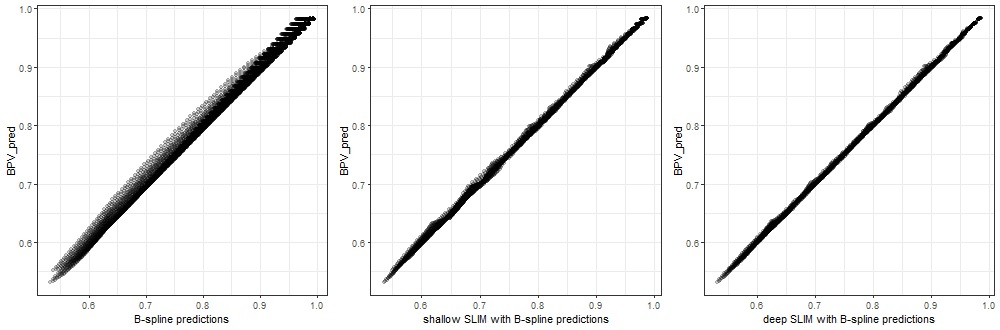
\includegraphics[width = 14cm]{Figures/insurance_use_case/k2204_BPV/fit.png}
    \caption{B-spline surrogate predictions vs. BPV\_pred for K2204}
    \label{fig:ins_k2204_fit}
\end{figure}

The fidelity results for all B-spline surrogates are listed in table \ref{tab:ins_k2204_bsplines_surrogates_perf} .

\begin{table}

\caption{Fidelity of K2204 B-spline baseline model and  B-spline MBTs}
\centering
\begin{tabular}[t]{l|r|r|r|r|r}
\hline
  & $R^2$ & MSE & MAE & max AE & n leaves\\
\hline
B-spline baseline model & 0.9943311 & 7.63e-05 & 0.0067811 & 0.0378568 & 1\\
\hline
SLIM shallow & 0.9994176 & 7.80e-06 & 0.0018244 & 0.0167730 & 8\\
GUIDE shallow & 0.9993900 & 8.20e-06 & 0.0019011 & 0.0165545 & 8\\
MOB shallow & 0.9992115 & 1.06e-05 & 0.0022236 & 0.0182034 & 8\\
CTree shallow & 0.9990918 & 1.22e-05 & 0.0024194 & 0.0183906 & 8\\
\hline
SLIM deep & 0.9997514 & 3.30e-06 & 0.0010766 & 0.0126778 & 21\\
GUIDE deep & 0.9997301 & 3.60e-06 & 0.0011730 & 0.0116453 & 20\\
MOB deep & 0.9996858 & 4.20e-06 & 0.0013448 & 0.0119785 & 21\\
CTree deep & 0.9997091 & 3.90e-06 & 0.0012936 & 0.0123686 & 20\\
\hline
\end{tabular}
\label{tab:ins_k2204_bsplines_surrogates_perf}
\end{table}


The improvement of the shallow MBTs over the baseline model is large, but not as substantial as in the trees with linear models without B-spline transformations. This is probably due to the fact that the splits in the MBTs with linear models also handled non-linearities that could not be adjusted in the linear baseline model. In the baseline model with B-spline transformations, on the other hand, the non-linearities are already taken into account and the splits then actually capture primarily the interactions, which is what is desired. 



Table \ref{tab:ins_k2204_bsplines_surrogates_share}  shows the proportions of observations that were split according to the different features. 


\begin{table}[!htb]
\caption{Share of observations split by the different features K2204 B-spline MBTs}
\centering
\begin{tabular}[t]{l|r|r|r}
\hline
  & Age & Duration & Sex\\
\hline
SLIM shallow & 0.38 & 0.62 & 0.00\\
GUIDE shallow & 0.30 & 0.70 & 0.00\\
MOB shallow & 0.08 & 0.84 & 0.08\\
CTree shallow & 0.23 & 0.71 & 0.07\\
\hline
SLIM deep & 0.35 & 0.60 & 0.04\\
GUIDE deep & 0.20 & 0.78 & 0.02\\
MOB deep & 0.08 & 0.76 & 0.16\\
CTree deep & 0.20 & 0.67 & 0.13\\
\hline
\end{tabular}
\label{tab:ins_k2204_bsplines_surrogates_share}
\end{table}

For SLIM, GUIDE and MOB the share results of the shallow trees are similar to the MBTs with linear models. Shallow CTree, on the other hand, selects Age in $23\%$ of split observations as splitting variable, whereas it was not used at all for splitting in CTree with linear models. It performs the worst in terms of fidelity in this case as well, but not as considerable as in the previous setting.

The deeper splitting improves the performance of all MBTs considerably. The MAE of the deep trees, for example, is only 52\%-61\% of the MAE of the shallow trees. CTree achieves the greatest improvement and thus comes close to the performance of the other MBTs. However, this better performance comes at the cost of interpretability. Additionally, there is an increased risk of overfitting.



For the interpretation, the shallow SLIM B-spline tree is analysed in more detail.

\begin{figure}[!htb]
    \centering   
    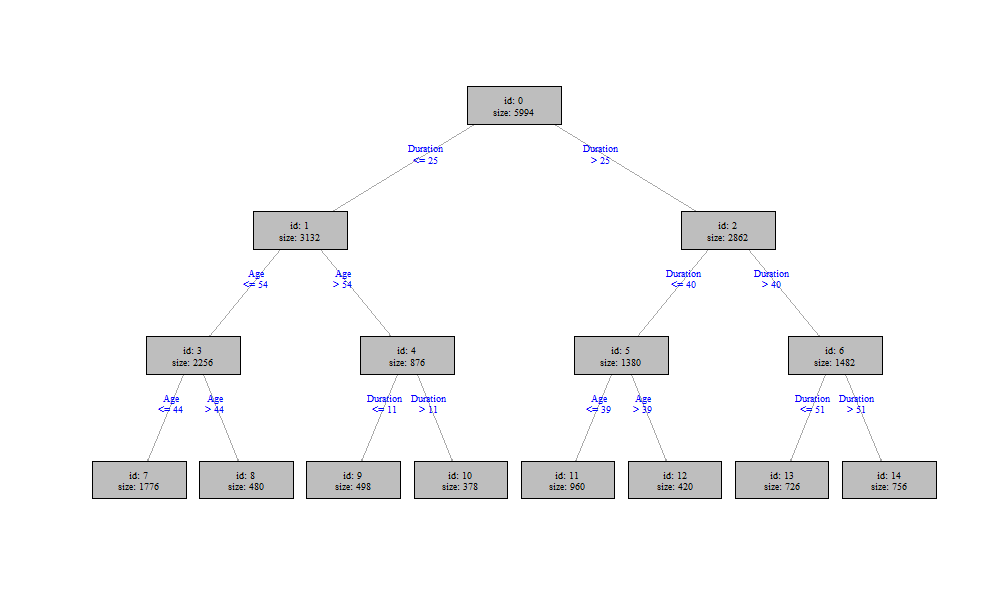
\includegraphics[width = 16cm]{Figures/insurance_use_case/k2204_BPV/slim_bsplines_small_tree.png}
         \caption{SLIM tree for K2204 with B-spline models}
     \label{fig:ins_slim_bsplines_tree}
\end{figure}

In order to investigate the effects of the splits on the feature effects more closely, the splits with regard to duration and age are analysed separately.
The nodes 1,5,13 and 14 together comprise the entire feature space, whereby the sub-regions are determined by splits with regard to the feature duration.
Figure \ref{fig:ins_k2204_effects_duration} shows the input-output relation (feature effects) of the features estimated in the B-spline models in the different nodes. Note that the effects are centred.

\begin{figure}[!htb]
    \centering
    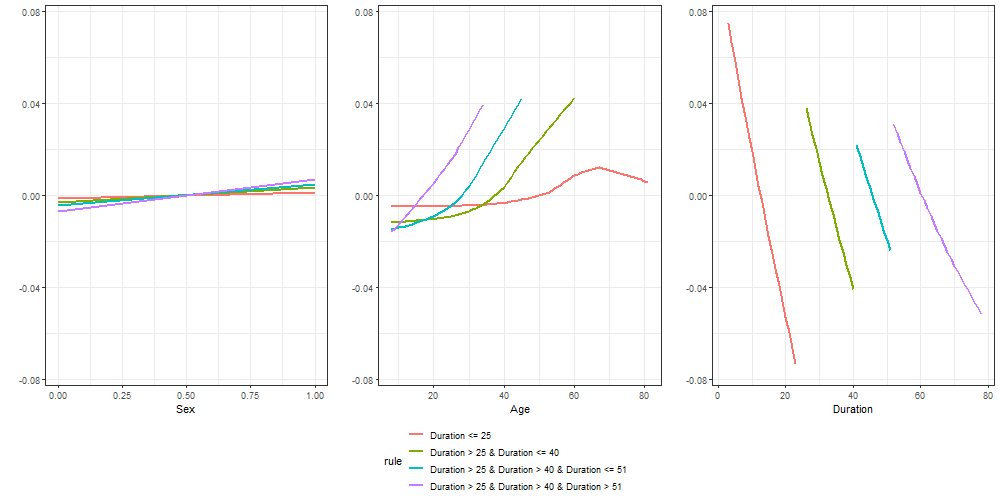
\includegraphics[width = 16cm]{Figures/insurance_use_case/k2204_BPV/effects_duration.png}
    \caption{Input-output relation of features in nodes split by duration for SLIM tree with B-splines and depth 3}
    \label{fig:ins_k2204_effects_duration}
\end{figure}

As with SLIM with linear models, it can be seen that the positive effect of Sex male increases with increasing duration. The same applies to Age. The seemingly negative effect of age at low maturity and high age is probably due to extrapolation. There are only a few observations in this area, as can be seen in Figure \ref{fig:ins_k2204_hist_age}.

\begin{figure}[!htb]
    \centering
    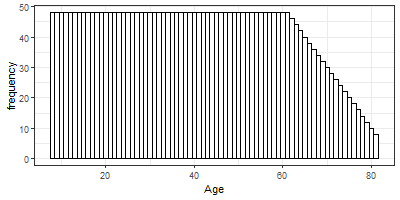
\includegraphics[width = 12cm]{Figures/insurance_use_case/k2204_BPV/hist_age.png}
    \caption{Frequency of observations with respect to feature Age}
    \label{fig:ins_k2204_hist_age}
\end{figure}

With the feature Duration, it can be seen that the negative effect decreases with increasing Duration.

To investigate the effect of splits with respect to feature Age, on the one hand nodes 4,7 and 8 are compared, which cover the featurespace for Duration $\leq 25$, and on the other hand nodes 11 and 12, which cover the featurespace for $25 > $Duration $<= 40$. In the Figures \ref{fig:ins_k2204_effects_age_low_duration} and \ref{fig:ins_k2204_effects_age_medium_duration} the corresponding input-output relations of the features are shown.

\begin{figure}[!htb]
    \centering    
    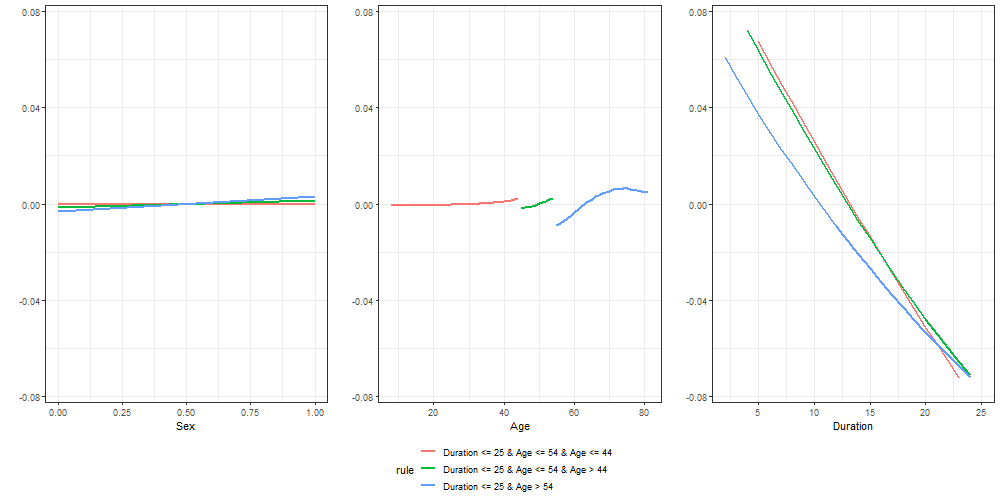
\includegraphics[width = 16cm]{Figures/insurance_use_case/k2204_BPV/effects_age_low_duration.png}
    \caption{Input-output relation of features in nodes with Duration $\leq 25$ split by Age for SLIM tree with B-splines and depth 3}
    \label{fig:ins_k2204_effects_age_low_duration}
\end{figure}

\begin{figure}[!htb]
    \centering    
    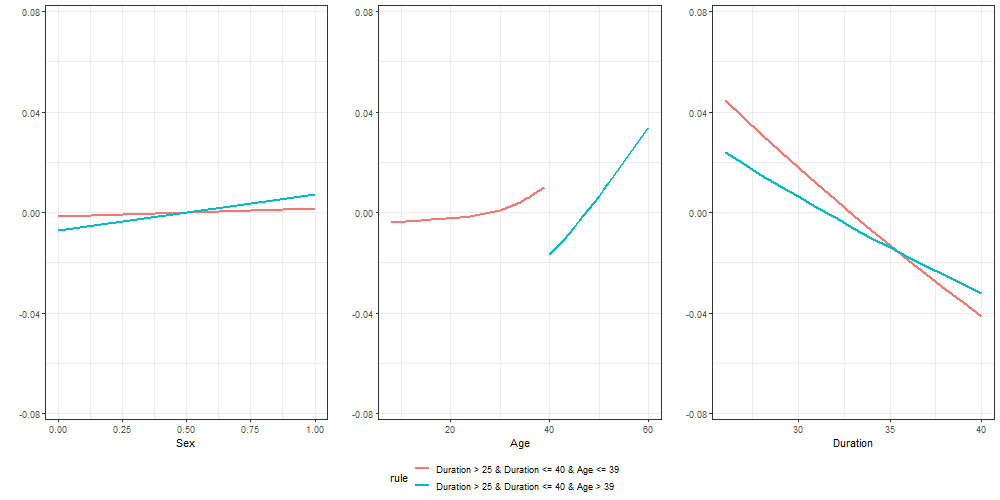
\includegraphics[width = 16cm]{Figures/insurance_use_case/k2204_BPV/effects_age_medium_duration.png}
    \caption{Input-output relation of features in nodes with $25 > $Duration $<= 40$ split by Age for SLIM tree with B-splines and depth 3}
    \label{fig:ins_k2204_effects_age_medium_duration}
\end{figure}

Again, the interpretation is consistent with the results from SLIM with linear models. The positive effect of sex times and age is increased by increasing age, while the negative effect of duration is reduced.The slightly negative effect of age at high age and low duration should again be viewed with caution and is probably due to the poor data situation in this area.


Finally, a deep SLIM tree with B-spline models is used as a standalone model for the prediction of BPV and its accuracy is compared to the accuracy of the black box model. The result is shown in Table \ref{tab:ins_k2204_standalone_slim}.
The accuracy of SLIM is worse than that of the black box model for all evaluation measures. However, the difference is most apparent for the max AE. While the max AE is explicitly minimised in the black box model, the MSE is minimised with SLIM. In general, a different loss function would also be possible with SLIM. In this case, either the max AE could be minimised only in the split selection, or also in the modelling in the nodes

\begin{table}[!htb]

\caption{Performance of baseline model and MBTs with bspline linear models}
\centering
\begin{tabular}[t]{l|r|r|r|r}
\hline
  & $R^2$ & MSE & MAE & max AE \\
\hline
SLIM & 0.9997757 & 3.1e-06 & 0.0010172 & 0.0118951\\
Blackbox model & 0.9998316 & 2.3e-06 & 0.0009441 & 0.0047668\\
\hline
\end{tabular}
\label{tab:ins_k2204_standalone_slim}
\end{table}








\subsection{Data set R1\_08}

The data set R1\_08 contains the data of an annuity insurance tariff. Instead of a single benefit in the endowment case, a lifelong annuity is paid out.
R1\_08 includes, in addition to sex, age and duration, the features birth\_year, payment\_period, in\_year\_payments\_exkasso (categorical with 4 levels), guarantee\_period and increment\_factor.
The value range of the features age and duration is limited to a range in which no correlation exists ($25 \leq$ age $\leq 35$ and $30 \leq$ Duration $\leq 40$).
Here, as well, the BPV or BPV\_pred is analysed as target variable. Here, as well, the BPV and BPV\_pred predicted by a black box model are analysed as target variables.
For the application of the MBTs, subsets of the training and test datasets including BPV and BPV\_pred are drawn, each with 100000 observations.

In order to model non-linearities in the nodes, MBTs with B-spline models are used. As with K2204, trees with two different depths are evaluated, shallow trees with a maximum depth of 3 and deep trees with a maximum depth of 7. $impr$ and $alpha$ are set to 0.05 and a minimum nodesize of 500 observations is required.

For the interpretation of the splits and models, the shallow SLIM tree is examined in more detail. Its structure is shown in Figure \ref{fig:ins_k108_slim_bsplines_small_tree}.

\begin{figure}[!htb]
    \centering
    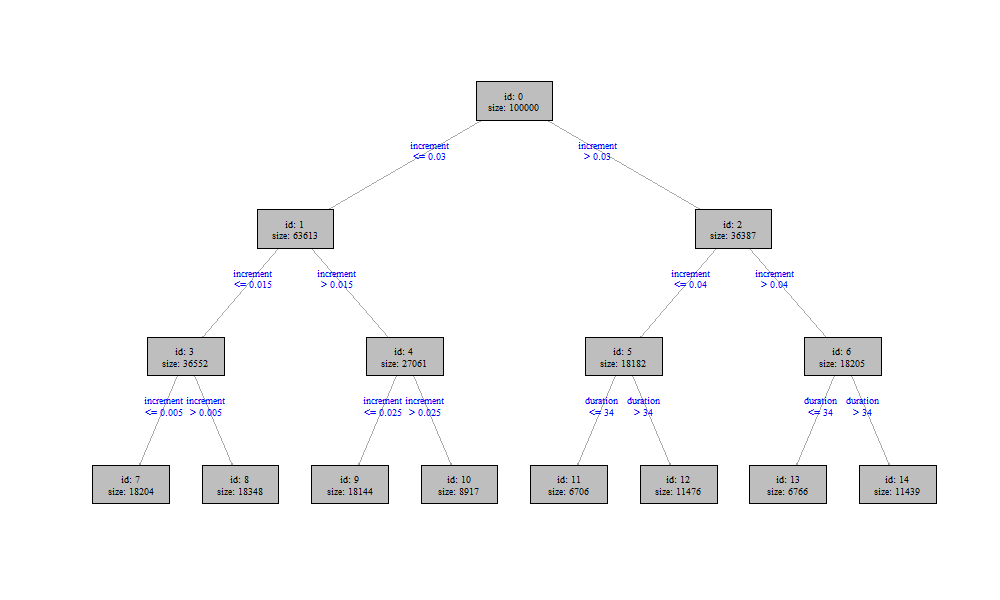
\includegraphics[width = 16cm]{Figures/insurance_use_case/k1_08_BPV/slim_bsplines_small_tree.png}
    \caption{Shallow SLIM tree for K1\_08 with B-spline models}
    \label{fig:ins_k108_slim_bsplines_small_tree}
\end{figure}

If the tree is fitted on the test data instead of the training data, exactly the same splits result. The same applies if the tree is used as a standalone model for BPV instead of a surrogate model. This indicates that the black box model replicates the true data and relationships well.
It is noticeable that the featurespace in the first splits is only divided iwith regard to increment\_factor. The effects of these splits on the other features are shown in Figure \ref{fig:ins_k108_effects_increment}.

\begin{figure}[!htb]
    \centering    
    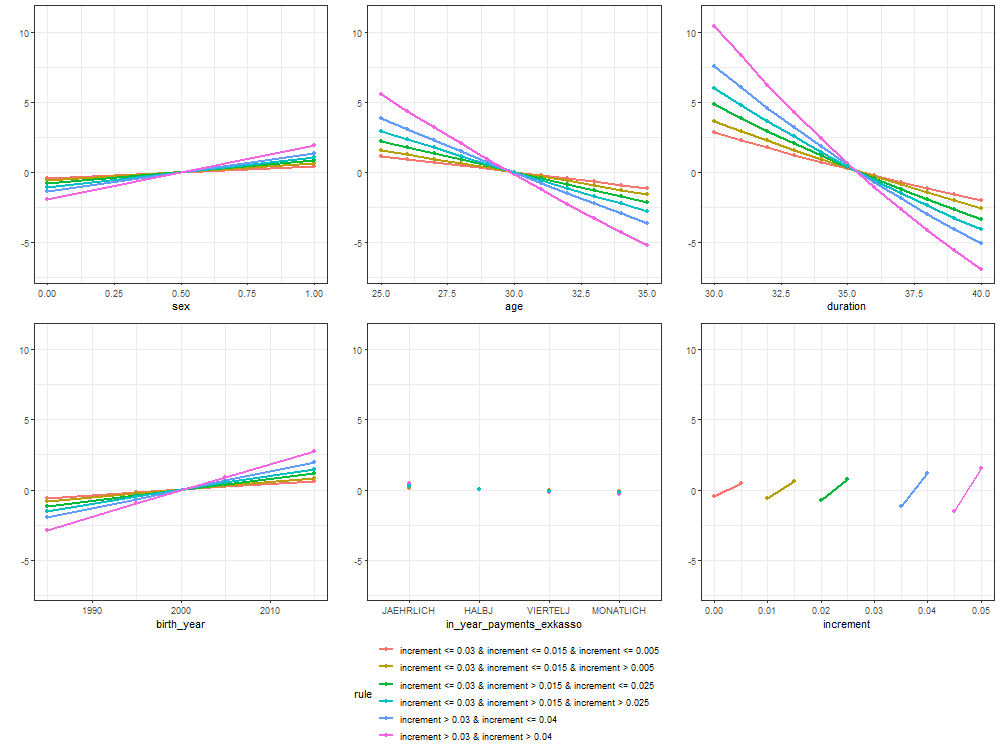
\includegraphics[width=16cm]{Figures/insurance_use_case/k1_08_BPV/effects_increment_factor.png}
    \caption{Input-output relation of features in nodes split by increment\_factor for SLIM tree with B-splines and depth 3}
    \label{fig:ins_k108_effects_increment}
\end{figure}

The effects of the features payment\_period and guarantee\_period are not shown because they are very small and therefore not visible on the scale at all.
The interaction with increment\_factor is clearly visible in all the features shown. For all features, an increasing increment\_factor increases the feature effects. Since increment factor interacts with so many features, the splits are very effective here and bring a great improvement in performance, as can be seen in table \ref{}.

The consequences of the splits with respect to duration are shown in Figure \ref{fig:ins_k108_effects_duration}. It shows that across all shown features a higher duration weakens the feature main effects.

\begin{figure}[!htb]
    \centering
    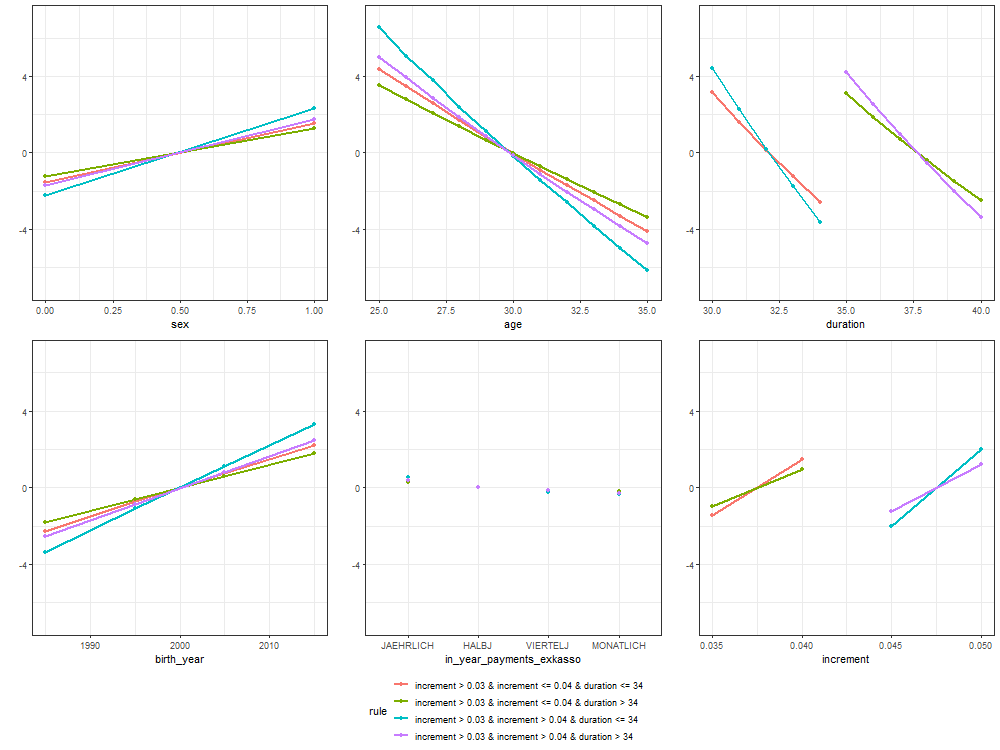
\includegraphics[width=16cm]{Figures/insurance_use_case/k1_08_BPV/effects_duration.png}
    \caption{Input-output relation of features in nodes split by Duration for SLIM tree with B-splines and depth 3 (nodes 11-14)}
    \label{fig:ins_k108_effects_duration}
\end{figure}






